\documentclass{article}
\usepackage[utf8]{inputenc}
\usepackage{amsmath}
\usepackage{amssymb}
\usepackage{graphicx}

\begin{document}

\section*{Conditional minimum with SVD}
Let $\mathbf{A} = \mathbf{U}\mathbf{\Sigma}\mathbf{V}^{\mathsf{T}}$ be the singular value decomposition of $\mathbf{A}\in \mathbb{C}^{m,n}$, $m \geq n$. Consider the following problem
\begin{equation}
    \mathbf{x}^{*} = \underset{\left\lVert \mathbf{x}\right\rVert_{2} = 1}{\text{argmin}}\left\{\left\lVert \mathbf{A}\mathbf{x}\right\rVert_{2}\right\}
\end{equation}
\subsection*{3-5.a} 
We are tasked with showing that the solution to (1) is given by $\mathbf{x}^{*} = \mathbf{v}_{n} := \mathbf{V}_{:,n}$. We have that $\mathbf{A} = \mathbf{U}\mathbf{\Sigma}\mathbf{V}^{\mathsf{T}}$ We know that both $\mathbf{U}$ and $\mathbf{V}$ are orthogonal matrices. For $\mathbf{x}$ with $\left\lVert \mathbf{x}\right\rVert_{2} = 1$ we have
\begin{equation*}
    \left\lVert \mathbf{A}\mathbf{x}\right\rVert_{2} = \left\lVert \mathbf{U}\mathbf{\Sigma}\mathbf{V}^{\mathsf{T}}\mathbf{x}\right\rVert_{2} = \left\lVert \mathbf{\Sigma}\mathbf{V}^{\mathsf{T}}\mathbf{x}\right\rVert_{2} 
\end{equation*}
Where we applied the following theorem on the preservation of euclidean norm.

\begin{figure}[!hbt]
    \centering
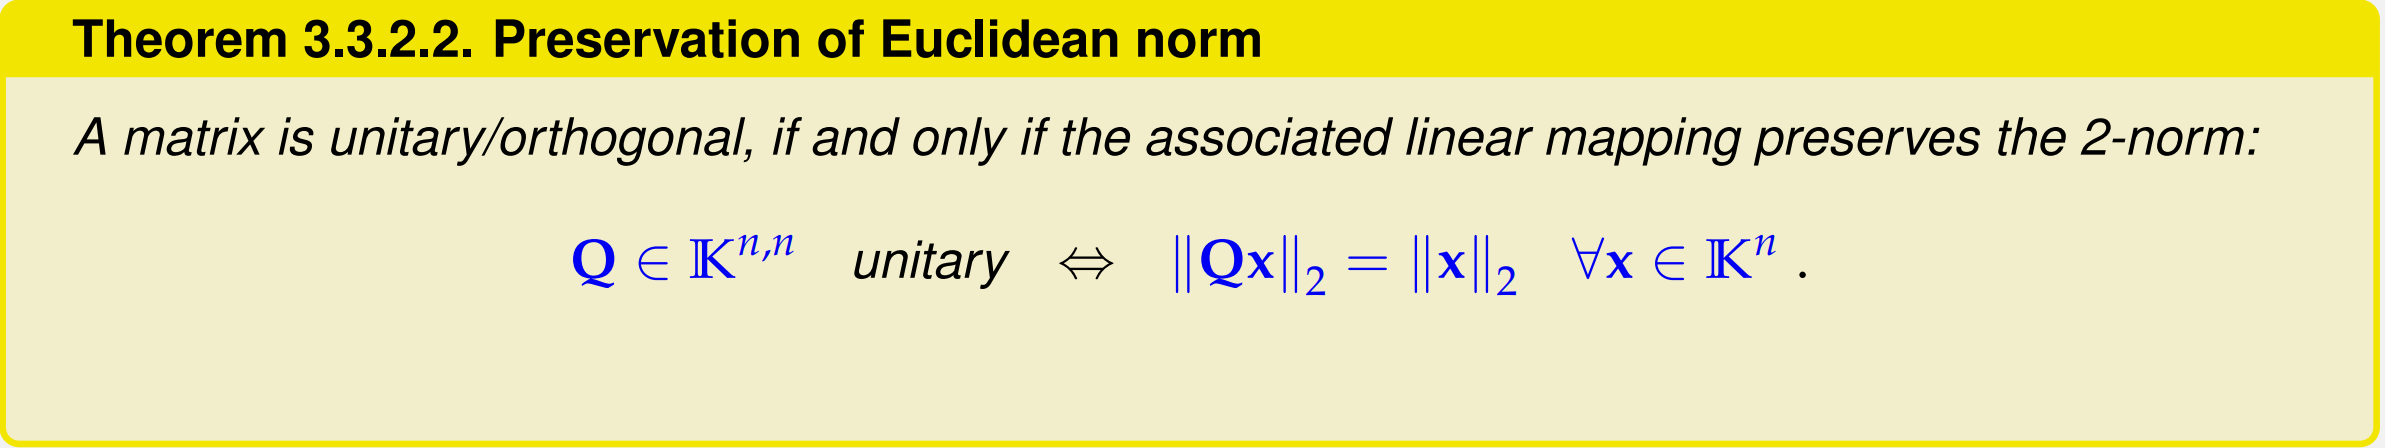
\includegraphics[width=1.0\linewidth]{PreservationEuclideanNorm.png}
\end{figure}

\noindent This follows from the orthogonality of $\mathbf{Q}$
\begin{equation*}
    \left\lVert \mathbf{Q}\mathbf{x}\right\rVert_{2} = \sqrt{\left(\mathbf{Q}\mathbf{x}\right)^{\mathsf{T}}\mathbf{Q}\mathbf{x}} = \sqrt{\mathbf{x}^{\mathsf{T}}\mathbf{Q}^{\mathsf{T}}\mathbf{Q}\mathbf{x}}  = \sqrt{\mathbf{x}^{\mathsf{T}}\left(\mathbf{Q}^{\mathsf{T}}\mathbf{Q}\right)\mathbf{x}} =\sqrt{\mathbf{x}^{\mathsf{T}}\mathbf{I}\mathbf{x}}
=\sqrt{\mathbf{x}^{\mathsf{T}}\mathbf{x}} = \left\lVert \mathbf{x}\right\rVert_{2}
\end{equation*}

\noindent Let us define $\mathbf{y} = \mathbf{V}^{\mathsf{T}}\mathbf{x}$, we see that because $\mathbf{V}$ is orthogonal we have $\left\lVert \mathbf{V}^{\mathsf{T}}\mathbf{x}\right\rVert_{2} =\left\lVert \mathbf{x}\right\rVert_{2} =1$. We hence write
\begin{equation*}
     \left\lVert \mathbf{A}\mathbf{x}\right\rVert_{2} =  \left\lVert \mathbf{\Sigma}\mathbf{V}^{\mathsf{T}}\mathbf{x}\right\rVert_{2}  =  \left\lVert \mathbf{\Sigma}\mathbf{y}\right\rVert_{2} 
\end{equation*}
We now use this to derive two inequalities which will then yield our desired result. We would want to have $x^{*} = \mathbf{v}_{n}$ which means that $\underset{\left\lVert x\right\rVert_{2} = 1}{\text{min}}\left\lVert \mathbf{A}\mathbf{x}\right\rVert_{2} = \sigma_{n}$. We firstly have
\begin{equation*}
    \underset{\left\lVert \mathbf{x}\right\rVert_{2} = 1}{\text{min}}\left\lVert \mathbf{A}\mathbf{x}\right\rVert_{2} = \underset{\left\lVert \mathbf{y}\right\rVert_{2} = 1}{\text{min}}\left\lVert \mathbf{\Sigma}\mathbf{y}\right\rVert_{2} = \underset{\left\lVert \mathbf{y}\right\rVert_{2} = 1}{\text{min}}\left\lVert \left[\sigma_{1}y_{1}, \dots, \sigma_{n}y_{n}\right]\right\rVert_{2} 
    = \underset{\left\lVert \mathbf{y}\right\rVert_{2} = 1}{\text{min}}\sqrt{\sigma_{1}^{2}y_{1}^{2} + \dots \sigma_{n}^{2}y_{n}^{2}}
\end{equation*}
We now apply that the singular values are sorted in descending order according to their absolute values. Hence we can write
\begin{equation*}
    \underset{\left\lVert \mathbf{y}\right\rVert_{2} = 1}{\text{min}}\sqrt{\sigma_{1}^{2}y_{1}^{2} + \dots \sigma_{n}^{2}y_{n}^{2}} \geq  \underset{\left\lVert \mathbf{y}\right\rVert_{2} = 1}{\text{min}}\sqrt{\sigma_{n}^{2}y_{1}^{2} + \dots \sigma_{n}^{2}y_{n}^{2}} = \sigma_{n}\underset{\left\lVert \mathbf{y}\right\rVert_{2} = 1}{\text{min}}\sqrt{y_{1}^{2} + \dots y_{n}^{2}} = \sigma_{n} \underset{\left\lVert \mathbf{y}\right\rVert_{2} = 1}{\text{min}} \left\lVert \mathbf{y}\right\rVert_{2}
\end{equation*}
Using that $\left\lVert \mathbf{y}\right\rVert = 1$ we hence can conclude that the last term above is equal to $\sigma_{n}$ and hence we have 
 \begin{equation*}
     \underset{\left\lVert \mathbf{y}\right\rVert_{2} = 1}{\text{min}}\sqrt{\sigma_{1}^{2}y_{1}^{2} + \dots \sigma_{n}^{2}y_{n}^{2}} \geq \sigma_{n}
 \end{equation*}

 \noindent On the other hand we have 
 \begin{equation*}
     \underset{\left\lVert \mathbf{y}\right\rVert_{2} = 1}{\text{min}}\sqrt{\sigma_{1}^{2}y_{1}^{2} + \dots \sigma_{n}^{2}y_{n}^{2}} = \underset{\left\lVert \mathbf{y}\right\rVert_{2} = 1}{\text{min}}\left\lVert \mathbf{\Sigma}\mathbf{y}\right\rVert_{2} 
 \end{equation*}
We now must make a suitable choice for an inequality $\leq$ such that we are able to derive $\sigma_{n}$ after some steps. We have $\sigma_{n} = \left(\mathbf{\Sigma}\right)_{n,n} = \mathbf{\Sigma} e_{n}$ and thus we do the following steps
\begin{equation*}
  \underset{\left\lVert \mathbf{y}\right\rVert_{2} = 1}{\text{min}}\left\lVert \mathbf{\Sigma}\mathbf{y}\right\rVert_{2}  \leq \left\lVert \mathbf{\Sigma}\mathbf{e}_{n}\right\rVert_{2} = \sigma_{n}  
\end{equation*}
The step is correct as we have $\left\lVert \mathbf{y}\right\rVert_{2} = 1$ and $\Sigma_{n}$ is the smallest singular value, hence the minimum will either be smaller or equal to $\mathbf{e}_{n}$ (equal is the case as we will prove). Overall we conclude
\begin{equation*}
   \underset{\left\lVert \mathbf{x}\right\rVert_{2} = 1}{\text{min}}\left\lVert \mathbf{A}\mathbf{x}\right\rVert_{2} = \sigma_{n} \implies \underset{\left\lVert \mathbf{x}\right\rVert_{2} = 1}{\text{argmin}}\left\lVert \mathbf{A}\mathbf{x}\right\rVert_{2} = \mathbf{e}_{n}
\end{equation*} 
Hence we get $\mathbf{y} = \mathbf{e}_{n} $, which gives us
\begin{equation*}
   \mathbf{y} = \mathbf{e}_{n} = \mathbf{V}^{\mathsf{T}}\mathbf{x} \implies \mathbf{x} = \mathbf{V}\mathbf{y} = \mathbf{V}\mathbf{e}_{n} = \mathbf{V}_{:,n} =: \mathbf{v}_{n}
\end{equation*}
Hence we have shown both statements.

\end{document}
